% Drawing 154/06-27 -- folder 154, batch 06, archive page 110 (PDF page 111).
% Transcription: au milieu de la page, dessins en couleur : un rectangle vert clair dont les côtés portent de petits traits rouges, marqués $n - \nu$ (grands côtés) et $\nu - 1$ (petits côtés), avec un « $2(\nu - 1)$ » entouré à côté ; un faisceau de droites rouges en étoile ; un rectangle $a\,b\,a'\,b'$ traversé de droites rouges qui se croisent, avec une ligne médiane en tirets ; à droite, une droite vert clair qui passe d'une hauteur à l'autre à travers un croisement de droites rouges, avec les points $a$, $a'$, $b$, $b'$ ; un rectangle vert clair aux coins marqués de petits carrés
% Kind: page of figures: ticked rectangles, star, strip a b a' b', a line changing level. Method 2 (schematic redraw from the facsimile). Status: ok.
% Notes: Six figures placed as on the page. The ticked rectangle (six ticks above, five below, four on each short side, a point at each upper corner, an arrow above, the circled 2(nu - 1) in pencil). The star of four red lines through one point, with an open pencil rectangle at its right. The strip a b a' b': brown upper side, light green lower side, a dashed red median, two crossings and two verticals between two K-shaped ends. The light green line passing from the lower level to the upper one through a red crossing, between a pencil line above and a dashed light green line below, with red strokes across (two on the left of the crossing, a horizontal arrowed one through it, one and a triple crossing on the right), a pencil rectangle round the crossing and the letters a', a, b, b'. A red cross with pencil brackets. The rectangle with a small square at each corner, ticks on its long sides, five red points on each short side and a pencil wedge outside each short side. Redrawn 2026-11-12 (issue 128): to check again. 2026-11-14, Claude Opus 5.5, overlay check (issue 147): rasterised from its own coordinates over the 400 dpi colour scan (402 ppi native) on a unit grid; not compiled (no TeX in the session). The six figures lie on their ink to within about 1 unit. Corrected: in the top right figure the lower level is pencil from the left end and light green only from x = 54.8 (the green ran from the left edge of the crop), and the upper pencil line carries light green dashes left of the pencil rectangle, now drawn; each pencil wedge outside the short sides of the lower rectangle is a bracket and a fan of four strokes from its apex, drawn so (they were two strokes); the small pencil oval at the upper left is added. Left out: a large faint pencil oval at the left edge, mostly outside the figure, and faint pencil scribbles under the top right figure. Status set to ok.
% Coordinates: 1 unit = 1 mm = 1/100 of the crop width (bbox in page fractions: [0.135, 0.215, 0.92, 0.455]).
% Redrawn by Claude (claude-fable-5-2), issue #128, 2026-11-12; not checked by a human; not compiled (no TeX in the session).
% Checked by Claude (claude-opus-5-5) 2026-11-14 (issue #147): overlaid on the 400 dpi colour facsimile; not compiled (no TeX in the session). Not checked by a human. Status: ok.
% Rights: reproduces part of the work -- behind RENDER_TRANSCRIPTS, never published by itself.
\documentclass[tikz,border=3pt]{standalone}
\usepackage{amsmath,amssymb}
\usetikzlibrary{patterns,arrows.meta}
\tikzset{Lg/.style={green!60!black!70}, Br/.style={brown!80!black}, Rd/.style={red!85!black}, pencil/.style={black!45}, struck/.style={black!35}, mpt/.style={circle,draw,inner sep=1.3pt}, pt/.style={circle,fill,inner sep=0.9pt}, opt/.style={circle,draw,fill=white,inner sep=1.1pt}}
\begin{document}
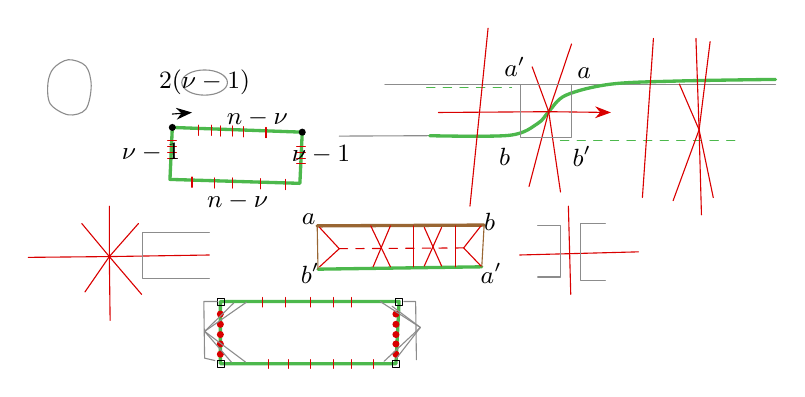
\begin{tikzpicture}[x=1mm,y=1mm,line cap=round,line join=round,font=\scriptsize]
\draw[Lg,very thick] (22.1,-11.9) -- (38.6,-12.5) -- (38.3,-19) -- (21.8,-18.5) -- cycle;
\draw[Rd] (25.4,-11.6) -- (25.4,-12.9);
\draw[Rd] (27.1,-11.6) -- (27.1,-12.9);
\draw[Rd] (28.2,-11.7) -- (28.2,-13);
\draw[Rd] (29.7,-11.7) -- (29.7,-13);
\draw[Rd] (31.1,-11.8) -- (31.1,-13.1);
\draw[Rd] (34,-11.9) -- (34,-13.2);
\draw[Rd] (24.6,-18.2) -- (24.6,-19.5);
\draw[Rd] (27.5,-18.3) -- (27.5,-19.6);
\draw[Rd] (29.7,-18.3) -- (29.7,-19.6);
\draw[Rd] (33.3,-18.4) -- (33.3,-19.7);
\draw[Rd] (36.5,-18.5) -- (36.5,-19.8);
\draw[Rd] (21.5,-13.6) -- (22.6,-13.6);
\draw[Rd] (21.5,-14.3) -- (22.6,-14.3);
\draw[Rd] (21.5,-15.1) -- (22.6,-15.1);
\draw[Rd] (21.5,-15.8) -- (22.6,-15.8);
\draw[Rd] (37.9,-14.3) -- (39,-14.3);
\draw[Rd] (37.9,-15.1) -- (39,-15.1);
\draw[Rd] (37.9,-15.8) -- (39,-15.8);
\draw[Rd] (37.9,-16.5) -- (39,-16.5);
\node[pt] at (22.1,-11.9) {};
\node[pt] at (38.6,-12.5) {};
\draw[-{Stealth[length=2mm]}] (22.1,-10.2) -- (24.6,-10);
\node[inner sep=1pt] at (32.9,-10.7) {\small $n-\nu$};
\node[inner sep=1pt] at (30.4,-21.3) {\small $n-\nu$};
\node[inner sep=1pt] at (19.4,-15.1) {\small $\nu-1$};
\node[inner sep=1pt] at (41,-15.4) {\small $\nu-1$};
\draw[pencil] (26.2,-6.2) ellipse[x radius=2.9, y radius=1.6];
\draw[pencil] plot[smooth cycle, tension=0.55] coordinates {(7,-4.4) (8.9,-3.3) (11.1,-4.1) (11.8,-6.6) (11.1,-9.6) (8.9,-10.3) (6.6,-8.9) (6.3,-6.3)};
\node[inner sep=1pt] at (26.2,-6.2) {\small $2(\nu-1)$};
\draw[Rd] (3.8,-28.4) -- (14.1,-28.3) -- (26.8,-28.1);
\draw[Rd] (14.1,-21.9) -- (14.1,-28.3) -- (14.2,-36.4);
\draw[Rd] (10.6,-24.1) -- (14.1,-28.3) -- (18.2,-33.1);
\draw[Rd] (17.8,-24.1) -- (14.1,-28.3) -- (11,-32.8);
\draw[pencil] (26.8,-25.2) -- (18.3,-25.2) -- (18.3,-31.1) -- (26.8,-31.1);
\draw[Br,very thick] (40.5,-24.4) -- (61.7,-24.3);
\draw[Lg,very thick] (40.6,-29.9) -- (61.4,-29.6);
\draw[Br] (40.5,-24.4) -- (40.6,-29.9);
\draw[Br] (61.7,-24.3) -- (61.4,-29.6);
\draw[Rd] (40.8,-24.6) -- (43.3,-27.3) -- (40.8,-29.6);
\draw[Rd] (61.3,-24.4) -- (59.1,-27.2) -- (61.3,-29.5);
\draw[Rd,dashed] (43.3,-27.3) -- (59.1,-27.2);
\draw[Rd] (47.3,-24.4) -- (49.8,-29.6);
\draw[Rd] (49.8,-24.4) -- (47.6,-29.6);
\draw[Rd] (54.1,-24.6) -- (56.3,-29.5);
\draw[Rd] (56.3,-24.6) -- (54.1,-29.5);
\draw[Rd] (52.7,-24.4) -- (52.7,-29.6);
\draw[Rd] (58.1,-24.4) -- (58.1,-29.6);
\node[inner sep=1pt] at (39.4,-23.6) {\small $a$};
\node[inner sep=1pt] at (62.4,-23.9) {\small $b$};
\node[inner sep=1pt] at (39.6,-30.4) {\small $b'$};
\node[inner sep=1pt] at (62.6,-30.4) {\small $a'$};
\draw[pencil] (49.1,-6.4) -- (98.7,-6.4);
\draw[pencil] (43.3,-13) -- (64.9,-12.9);
\draw[Lg,dashed] (54.4,-6.8) -- (65.2,-6.8);
\draw[Lg,very thick] plot[smooth, tension=0.55] coordinates {(54.8,-12.95) (64.9,-12.9) (68.5,-11.4) (69.9,-9.9) (72.1,-7.8) (77.8,-6.4) (86.5,-6) (98.7,-5.8)};
\draw[Lg,dashed] (71.4,-13.6) -- (93.7,-13.6);
\draw[Rd] (62.2,0.7) -- (59.9,-21.9);
\draw[Rd] (72.8,-1.3) -- (69.9,-9.9) -- (67.4,-19.4);
\draw[Rd] (67.8,-4.2) -- (69.9,-9.9) -- (71.4,-20.1);
\draw[Rd,-{Stealth[length=2mm]}] (55.9,-10) -- (69.9,-9.9) -- (77.8,-10);
\draw[Rd] (83.2,-0.6) -- (81.8,-20.8);
\draw[Rd] (88.6,-0.6) -- (89,-12.2) -- (89.3,-23);
\draw[Rd] (90.4,-1) -- (89,-12.2) -- (85.7,-21.2);
\draw[Rd] (86.5,-6.4) -- (89,-12.2) -- (90.8,-20.8);
\draw[pencil] (66.3,-6.4) -- (72.8,-6.4) -- (72.8,-13.2) -- (66.3,-13.2) -- cycle;
\node[inner sep=1pt] at (65.6,-4.2) {\small $a'$};
\node[inner sep=1pt] at (74.4,-5) {\small $a$};
\node[inner sep=1pt] at (64.3,-15.6) {\small $b$};
\node[inner sep=1pt] at (74.1,-15.6) {\small $b'$};
\draw[Rd] (66.2,-28.1) -- (81.3,-27.7);
\draw[Rd] (72.4,-21.9) -- (72.7,-33.1);
\draw[pencil] (68.5,-24.4) -- (71.4,-24.4) -- (71.4,-30.9) -- (68.5,-30.9);
\draw[pencil] (77.1,-24.1) -- (73.9,-24.1) -- (73.9,-31.3) -- (77.1,-31.3);
\draw[Lg,very thick] (28.2,-34) -- (50.9,-34) -- (50.5,-41.9) -- (28.2,-41.9) -- cycle;
\draw[Rd] (33.6,-33.5) -- (33.6,-34.7);
\draw[Rd] (36.5,-33.5) -- (36.5,-34.7);
\draw[Rd] (39.7,-33.5) -- (39.7,-34.7);
\draw[Rd] (42.6,-33.5) -- (42.6,-34.7);
\draw[Rd] (44.8,-33.5) -- (44.8,-34.7);
\draw[Rd] (34.3,-41.4) -- (34.3,-42.5);
\draw[Rd] (36.9,-41.4) -- (36.9,-42.5);
\draw[Rd] (39.7,-41.4) -- (39.7,-42.5);
\draw[Rd] (42.6,-41.4) -- (42.6,-42.5);
\draw[Rd] (44.8,-41.4) -- (44.8,-42.5);
\draw[Rd] (47.6,-41.4) -- (47.6,-42.5);
\node[pt,Rd] at (28.2,-35.6) {};
\node[pt,Rd] at (28.2,-36.9) {};
\node[pt,Rd] at (28.2,-38.2) {};
\node[pt,Rd] at (28.2,-39.4) {};
\node[pt,Rd] at (28.2,-40.7) {};
\node[pt,Rd] at (50.5,-35.6) {};
\node[pt,Rd] at (50.5,-36.9) {};
\node[pt,Rd] at (50.5,-38.2) {};
\node[pt,Rd] at (50.5,-39.4) {};
\node[pt,Rd] at (50.5,-40.7) {};
\draw (27.8,-33.6) -- (28.7,-33.6) -- (28.7,-34.5) -- (27.8,-34.5) -- cycle;
\draw (50.4,-33.6) -- (51.3,-33.6) -- (51.3,-34.5) -- (50.4,-34.5) -- cycle;
\draw (50.1,-41.5) -- (50.9,-41.5) -- (50.9,-42.4) -- (50.1,-42.4) -- cycle;
\draw (27.8,-41.5) -- (28.7,-41.5) -- (28.7,-42.4) -- (27.8,-42.4) -- cycle;
\draw[pencil] (27.8,-34) -- (26.1,-34) -- (26.2,-41.2) -- (27.5,-41.5);
\draw[pencil] (29.9,-34.2) -- (26.2,-37.8) -- (29.6,-41.7);
\draw[pencil] (31.5,-34.1) -- (26.2,-37.8) -- (31.4,-41.7);
\draw[pencil] (51.5,-34) -- (53,-34) -- (53.1,-41.4);
\draw[pencil] (48.5,-34) -- (53.6,-37.3) -- (49,-41.6);
\draw[pencil] (50,-34.6) -- (53.6,-37.3) -- (50.5,-41.3);
\end{tikzpicture}
\end{document}
